%% Template for MLP Coursework 2 / 25 November 2022

%% Based on  LaTeX template for ICML 2017 - example_paper.tex at 
%%  https://2017.icml.cc/Conferences/2017/StyleAuthorInstructions

\documentclass{article}
\usepackage[T1]{fontenc}
\usepackage{amssymb,amsmath}
\usepackage{txfonts}
\usepackage{microtype}

% For figures
\usepackage{graphicx}
\usepackage{subcaption} 

% For citations
\usepackage{natbib}

% For algorithms
\usepackage{algorithm}
\usepackage{algorithmic}

% the hyperref package is used to produce hyperlinks in the
% resulting PDF.  If this breaks your system, please commend out the
% following usepackage line and replace \usepackage{mlp2017} with
% \usepackage[nohyperref]{mlp2017} below.
\usepackage{hyperref}
\usepackage{url}
\urlstyle{same}

\usepackage{color}
\usepackage{booktabs} % To thicken table lines
\usepackage{multirow} % Multirow cells in table

% Packages hyperref and algorithmic misbehave sometimes.  We can fix
% this with the following command.
\newcommand{\theHalgorithm}{\arabic{algorithm}}


% Set up MLP coursework style (based on ICML style)
\usepackage{mlp2022}
\mlptitlerunning{MLP Coursework 2 (\studentNumber)}
\bibliographystyle{icml2017}
\usepackage{bm,bbm}
\usepackage{soul}

\DeclareMathOperator{\softmax}{softmax}
\DeclareMathOperator{\sigmoid}{sigmoid}
\DeclareMathOperator{\sgn}{sgn}
\DeclareMathOperator{\relu}{relu}
\DeclareMathOperator{\lrelu}{lrelu}
\DeclareMathOperator{\elu}{elu}
\DeclareMathOperator{\selu}{selu}
\DeclareMathOperator{\maxout}{maxout}
\newcommand{\bx}{\bm{x}}




\definecolor{red}{rgb}{0.95,0.4,0.4}
\definecolor{blue}{rgb}{0.4,0.4,0.95}
\definecolor{orange}{rgb}{1, 0.65, 0}

\newcommand{\youranswer}[1]{{\color{red} \bf[#1]}} %your answer: 


%% START of YOUR ANSWERS
%% REPLACE sXXXXXXX with your student number
\def\studentNumber{s2298839}


%% START of YOUR ANSWERS
%% Add answers to the questions below, by replacing the text inside the brackets {} for \youranswer{ "Text to be replaced with your answer." }. 
%
% Do not delete the commands for adding figures and tables. Instead fill in the missing values with your experiment results, and replace the images with your own respective figures.
%
% You can generally delete the placeholder text, such as for example the text "Question Figure 3 - Replace the images ..." 
%
% There are 5 TEXT QUESTIONS. Replace the text inside the brackets of the command \youranswer with your answer to the question.
%
% There are also 3 "questions" to replace some placeholder FIGURES with your own, and 1 "question" asking you to fill in the missing entries in the TABLE provided. 
%
% NOTE! that questions are ordered by the order of appearance of their answers in the text, and not necessarily by the order you should tackle them. You should attempt to fill in the TABLE and FIGURES before discussing the results presented there. 
%
% NOTE! If for some reason you do not manage to produce results for some FIGURES and the TABLE, then you can get partial marks by discussing your expectations of the results in the relevant TEXT QUESTIONS. The TABLE specifically has enough information in it already for you to draw meaningful conclusions.
%
% Please refer to the coursework specification for more details.


%% - - - - - - - - - - - - TEXT QUESTIONS - - - - - - - - - - - - 

%% Question 1:
\newcommand{\questionOne} {
\youranswer{
    According to Figure1, as the number of epochs increases, the training and Validation 
    loss of VGG08 decreases while training and Validation accuracy increases. However,
    the the training and Validation loss of VGG38 remain the same, and the training and 
    Validation accuracy of VGG38 stay at 0, which means the model of VGG38 has no 
    improvement in the training process. 

    According to Figure2 and Figure3, the absolute mean gradient of VGG08 can be passed 
    to the input layer. While the gradient of VGG38 only has positive values around the 
    output layer, and no gradient is passed to the input layer through backpropogation. 
    So the VGG38 model suffers from Vanishing Gradient Problem. 

    The consequences dipicted are that when simply stacking layers in network(VGG38 here) 
    the gradient of layers(expect the last few layers) will vanish, resulting that the 
    model can not be updated(due to 0 grad), and the model will lose the ability to 
    learn(convergence to a low error and high accuracy relative to the initial training period). 
}
}

%% Question 2:
\newcommand{\questionTwo} {
\youranswer{
    According to Table1, Figure2 and Figure3 in CW1, when the network capacity(depth or width) increases, 
    the model will suffer from overfitting, in which case the gap between training error and validation(or test) 
    error will be bigger, and the gap between training accuracy and validation(or test) accuracy will also become 
    bigger. This means when overfitting happens, the trained model will have a good performance on fitting the 
    training data, but having a relatively poor ability to fit the validation(or test) data(it can be reflected 
    on the gap between training and validation error(and acc) curves, when network capacity increases, gap bigger).\\ 
    But considering the results of Figure1. The gap between training and validation error 
    is not increasing when network capacity increases, but rather the network having deeper 
    layers(38 to 8) will have higher training error and lower training accuracy. 

    Also considering the Figure1 from \cite{he2016deep}. Both training and validation error of 
    56-layer plain network are higher than 20-layer network, but the gap between training error 
    and validation error is not increasing as network capacity increases(depth grows), and 
    the trend performs the same in Figure4(left) from \cite{he2016deep}. This means overfitting 
    does not happen. 

    The problem of vanishing gradients leads to the worse performance on deeper network. It 
    happens at the beginning of convergence. When the network depth increases, accuracy 
    gets saturated and then degrades(not caused by overfitting), which generate higher 
    training error.

}
}

%% Question 3:
\newcommand{\questionThree} {
\youranswer{
    In \cite{ioffe2015batch} it describes the goal of the Batch Normalisation is to 
    solve the problem of Internal Covariate Shift by unifying the distribution of 
    data in each mini-batch(too costly to fully whitening the inputs of one layer). 
    Assunming that values of $x$ over a mini-batch with size $m$,
    $\mathcal{B} = {x_{1...m}}$. The output ${y_i = BN_{\gamma,\beta}(x_i)}$ with 
    parameters $\gamma, \beta$ to be learned. 

    The procedure of Batch Normalisation Transform is as below.\\
    The first step is to calculate the mean and variance on each column(feature)  
    
        $\mu_{\mathcal{B}} = \frac{1}{m}\sum_{i=1}^{m}x_i \qquad
        \sigma_{\mathcal{B}}^2 = \frac{1}{m}\sum_{i=1}^{m}(x_i - \mu_{\mathcal{B}})^2$

    Then perform normalization on $x_i$

        $\hat{x}_i = \frac{x_i - \mu_{\mathcal{B}}}{\sqrt{\sigma_{\mathcal{B}}^2 + \epsilon}}$
    
    where $\epsilon$ is a constant added to mini-batch variance for numerical stability.
    If $\epsilon$ is neglected, the normalized activations will have same mean of $0$ and 
    variance of $1$ at training time.\\
    Finally $y_i$ is computed as a linear transformation of $x_i$ as 

        $y_i = \gamma x_i + \beta \equiv BN_{\gamma,\beta}(x_i)$

    

    When considering the training and testing of Batch Normalisation networks. The 
    $x$ inputed to one layer is now transformed to $BN(x)$. Both batch gradient descent and 
    SGD with mini-batch can be used to do the training. 
    
    The complete procedure of training and testing(validating, inference) a BN network is shown below.\\
    Considering the inputs are the network $N$ with trainable parameters $\Theta$ and 
    subset of activations $\{x^{(k)}\}^K_{k=1}$, the outputs are trained BN network for 
    testing $N^{inf}_{BN}$

    The first step is to train the network $N^{tr}_{BN}$ from $N$. So on each column(feature) 
    $k$, add the transformation $y^{(k)} = BN_{\gamma^{(k)}, \beta^{(k)}}(x^{(k)})$ to $N^{tr}_{BN}$ 
    as the transform shown above. Then modify each layer in $N^{tr}_{BN}$ 
    with input $x^{(k)}$ to take $y^{(k)}$ instead. After the for-loop, Train $N^{tr}_{BN}$ 
    to optimize the parameters $\Theta$ and $\{\gamma^{(k)}, \beta^{(k)}\}^K_{k=1}$

    After the training period, the trained network $N^{tr}_{BN}$ will be transformed to 
    $N^{inf}_{BN}$ for testing by freezing its parameters.  \\ 
    Because the normalization of activations
    (depending on mini-batch data) is not needed during test time(the output should depend only on the input). So when the 
    network has beed trained, the normalization should not contain mean and variance of one 
    specific mini-batch, instead, population(mean and variance of the whole input) is used.

        $\hat{x}^{(k)} = \frac{x^{(k)} - E[x^{(k)}]}{\sqrt{Var[x^{(k)}] + \epsilon}}$

    On each column(feature) $k$, to obtain the $E[x^{(k)}]$ and $Var[x^{(k)}]$, we should 
    process multiple training mini-batches $\mathcal{B}$, each of size $m$, and average over 
    them. 
    
        $E[x^{(k)}] = E_{\mathcal{B}}[\mu_{\mathcal{B}}^{(k)}]$ 
        \qquad
        $Var[x^{(k)}] = \frac{m}{m-1}E_{\mathcal{B}}[{\sigma_{\mathcal{B}}^{(k)}}^2]$ 

    Upon $\hat{x}^{(k)}$ is obtained. In $N^{inf}_{BN}$, replace the transform  
    $y^{(k)} = BN_{\gamma^{(k)}, \beta^{(k)}}(x^{(k)})$ with 
    $y^{(k)} = \gamma^{(k)} x^{(k)} + \beta^{(k)}$

    The Batch Normalisation transforms the inputs of activation to 
    Standard Normal Distribution, which prevents the data to move to the saturated region 
    of the nonlinear activations(it will cause the gradient to vanish). For example, 
    \cite{ioffe2015batch} mentioned the sigmoid activation will suffer from vanishing gradient 
    if not using BN in deep network. Also, network with Batch Normalisation can have higher 
    learning rate(because the learning rate value does not affect the backpropogation), 
    which will to some extent prevent the problem of gradient vanishing. 

}
}

%% Question 4:
\newcommand{\questionFour} {
\youranswer{
    \textit{Eqn.(1).} in \cite{he2016deep} explains that the input $x$ and $\mathcal{F}$ 
    must be of same dimension so that the output $y$ can be the sum of them. When 
    downsampling is applied, by which the dimension of $\mathcal{F}(x, \{W_i\})$ is changed, 
    the dimension of $x$ must also be changed to the same as $\mathcal{F}$ in order to 
    add residual connections to the downsampling layers. 

    One way to solve the dimension mismatch problem to use zero-padding shortcuts. For example the input of one block has 
    64 feature map dimension, while the output has 128. Then zero-padding can be performed 
    on the input to increase dimension to 128 and match the size of the output. 

    Another way is to use a projection shortcuts. 
    According to \textit{Eqn.(2).} in \cite{he2016deep}, a linear projection $W_j$ can be 
    performed on $x$ to fit the size of $\mathcal{F}$, so the output $y = \mathcal{F} + W_jx$ 

    Considering the pros and cons of these 2 solutions. The strengths of zero-padding is 
    that it is parameter-free(no additional parameters exist when padding), which can ensure 
    a relatively small size of the model(low network capacity). This can reduce training time 
    complexity(less parameters to calculate) and prevent 
    overfitting(based on the results in CW1 of the relationship between network capacity and overfitt).
    While the shortcomings of zero-padding is that it indeed has no residual 
    learning, instead just adding $0$ 
    to fit the output dimension, which can result in the relatively bad performance on 
    the trained model(based on Table3 in \cite{he2016deep}) compared to projection shortcuts.
    
    The advantages of projection is that extra parameters are introduced into the network by 
    projection shortcuts, and with the help of residual learning through 
    backpropogation(brought by parameters for projection),
    the network can fit a more complex model/distribution in deep learning, which 
    ensures a relatively lower training and validation error and higher accuracy(Table3 in \cite{he2016deep}). 
    While the disadvantages of projection is that the additional parameters need more time to 
    train and more space to save the network, which increases the time/memory complexity. For 
    example in bottleneck architecture described in \cite{he2016deep}, the parameters will be 
    doubled if replacing identify shortcuts with projection. Also, in deep network, the parameters in 
    projection may hamper information propagation and lead to optimization problems. Moreover, 
    the increse of network can cause overfitting problem in some cases.

}
}


%% Question 5:
\newcommand{\questionFive} {
\youranswer{
    Comparing the experiment results in Table1. The VGG08 plain trained model has $60 K$ parameters, 
    VGG38 plain trained model has $336 K$ parameters. When using BN on VGG38, the number of parameters 
    will increase by about $3 K$, while using RC does not affect it. Assunming the better 
    performance means higher Train and Val acc, with lower Train and Val loss.
    \begin{itemize}
        \item Plain network: When comparing VGG08 to VGG38 without BN or RC, the performance 
        of VGG08 overwhelm that of VGG38. The VGG38 suffer from problem of gradient 
        vanishing(Figure 1,2,3) because of the zero gradient and zero trainin and validation accuracy.
        \item The influence of BN and RC: 
        When only using BN for the broken VGG38, the performance 
        of it is a little bit better than VGG08. When only using RC for broken VGG38, the 
        performance is better than that of only using BN. This means either BN or RC can 
        to some extent solve the problem of gradient vanishing in deep network. Though using 
        RC can ensure better performance, yet the gap between Train(both loss and acc) and Val 
        will be bigger than using BN alone and VGG08, which means there exists some overfitting 
        problem in VGG38+RC network. 
        
        When combining BN and RC, the performance of VGG38 BN+RC 
        improves a little compared to using RC alone, moreover, the overfitting problem is slightly 
        alleviated(gap between train and val decreases). What can be inferred is that both 
        BN and RC can handle the problem of gradient vanishing, BN is helpful is releasing the 
        problem of overfitting, while RC ensures the network a better performance. Morever, 
        VGG38 BN+RC can combine their strengths(low loss high acc, and the gap between train 
        and val will not be too large).
        \item Change of learning rate: The performance of VGG38 BN with 1e-3 
        LR is slightly better than that of VGG38 BN with 1e-2 LR, which means the BN can maintain 
        the resilience of model to the LR scale. The small decrease 
        in Val accuracy of large learning rate is also corresponding to 
        Figure2(BN-x5 better than BN-x30) in \cite{ioffe2015batch}. 
        
        However, the performance of 
        VGG38 BN+RC with 1e-2 LR improves a lot compared to VGG38 BN+RC with 1e-3 
        LR(the best trained model so far). This may be because when LR increases, both BN and RC can 
        make the model converge faster, so the VGG38 BN+RC with 1e-2 LR can achieve much better 
        performance than the same model with 1e-3 LR within $100$ epochs.
    \end{itemize}

    According to Figure4, the training curve of the best trained model VGG38 BN+RC with 1e-2 LR. 
    It can be viewed that the validation error, though fluctuating, converges after epoch 80.
    And considering the Figure5, the gradient of each bn layer is not zero, while the 
    gradient of convolutional layers are zero. So it indicates that the Batch Normalisation 
    layers help the model to pass gradient through backpropogation, which solves the 
    problem of vanishing gradient.

    The further experiments can be planned as follows:
    \begin{itemize}
        \item Firstly, train the model of VGG08 BN, VGG08 RC, VGG08 BN+RC(the same 
        as VGG38) with 1e-3 LR, to demonstrate what is the best trained model(just like we have 
        selected the best trained model using VGG38 is VGG38 BN+RC).
        \item Secondly, after selecting the setting of 
        the best trained model based on VGG08 and VGG38
        (maybe VGG08 BN+RC and VGG38 BN+RC), choose different 
        LR(like Figure2 in \cite{ioffe2015batch}), for example, 1e-4, 5e-4, 5e-3, 5e-2, to test 
        what LR is best suitable for the two settings. 
    \end{itemize}
        So in the first step, we selected the best combination of BN and RC on VGG08, then 
        we test different learning rate to find the best LR. If in the first step, the best 
        trained model is VGG08 plain, then we need extra experiments(do step two) on the 
        settings which performs only worse than VGG08 plain in step one. Because since we have 
        the prior knowledge(also can be inferred from previous experiments) that the plain 
        network is sensitive to learning rate, so if the 1e-3 LR happens to be best suitable for 
        plain network, then step two on only plain VGG08 is futile(the best performance maybe 
        in VGG08 BN+RC with some other LR)

        After that we shall do some experiments on learning about the behaviour of BN and RC.
    \begin{itemize}
        \item Firstly, we want to know in BN networks, whether 
        the gradient value is negatively correlated to 
        the LR(Since \cite{ioffe2015batch} has described that the increase of LR will cause 
        the increase of parameter scale, and large parameters scale generates small gradients).
        So I will use either VGG08 BN or VGG38 BN(no RC, only study BN) with different 
        LR(like 1e-4, 5e-4, 5e-3) and plot the gradient flow.
        \item Secondly, we want to know in RC networks, the different performance between 
        zero-padding shortcuts and projection shortcuts on downsampling 
        layers(including time/memory cost, val accuracy) and weighing the pros and cons of 
        the two shortcuts to arrive at the most suitable combination. 
        So I will use two VGG38 RC(no BN, only study RC), one with zero-padding on its downsampling 
        layers, another with projection on its downsampling layers. Train them and compare the 
        running time, memory used and val accuracy. 
    \end{itemize}

}
}

%% Question 6:
\newcommand{\questionSix} {
\youranswer{
    We firstly find the vanishing gradient problem(VGP) in VGG38 network. Then we go over 
    the theory of 2 typical methods BN(\cite{ioffe2015batch}) and RC(\cite{he2016deep}), 
    which help solve VGP. Then we do experiments 
    on VGG38 with several combination of BN and RC. 
    By comparing the performance and gradient flow of them, we conclude that the 
    BN and RC is of help in solving VGP.
    The trained model with best performance in out 
    experiments in VGG38 BN+RC with 1e-2 LR. 

    The introduction of shortcuts in RC \cite{he2016deep} prevents the gradient 
    flow in deep network not to reducing to $0$, thus maintain the update of network. While 
    the bn layers in BN network \cite{ioffe2015batch} normalize the input mini-batch, 
    which enables layers share the same distribution, thus 
    reducing internal covariate shift. 
    The normalization also helps keep the layer input at the non-saturated region of the 
    activation layers, which prevents VGP.
    The bn layers can also maintain the resilience of the network to parameter scale, thus 
    large LR can be used.

    Some of our experiments demonstrates same trend with others. Like the VGG38 BN with 1e-3 LR 
    compared to VGG38 BN with 1e-2 LR. It shows similar results with Figure2 in \cite{ioffe2015batch}, 
    the BN-x5 and BN-x30. 
    
    Either BN or RC can handle 
    VGP. BN has additional effect on solving overfitting 
    problems(gap of using BN alone between train and val is bigger than that of using RC alone) 
    while RC ensures 
    a better performance of the trained 
    model(in Table1, the performance of using RC alone is better than that of using BN alone), 
    and both of them can increase the resilience 
    of the network to big learning rate(LR). 

    Considering the future work, we could increase the number of layers in 
    the RC network, and then test whether BN can help solve the problem of overfitting by 
    using one network with RC+BN while the other with RC alone. 

    Inspired by \cite{ioffe2015batch}, when the size of training data is extremely large, 
    the batch normalization need a big batch to enable its accurate approximation 
    of the global mean and global variance, which put pressure on hardware. 
    So is there an alternative that can help reduce hardware requirements for training.
    Also, when each input instance in a batch varies from each other a lot, the BN may 
    not help because it only computes the mean value within a batch. We can try to realize 
    the instance normalization by only calculate the mean of one instance. 

}
}

%% - - - - - - - - - - - - FIGURES - - - - - - - - - - - - 

%% Question Figure 3:
\newcommand{\questionFigureThree} {
\youranswer{Question Figure 3 - Replace this image with a figure depicting the average gradient across layers, for the VGG38 model.

\textit{(The Figure we give is correct, and can be used in your analysis. It is partially obscured so you can get credit for producing your own copy).}
%
\begin{figure}[t]
    \centering
    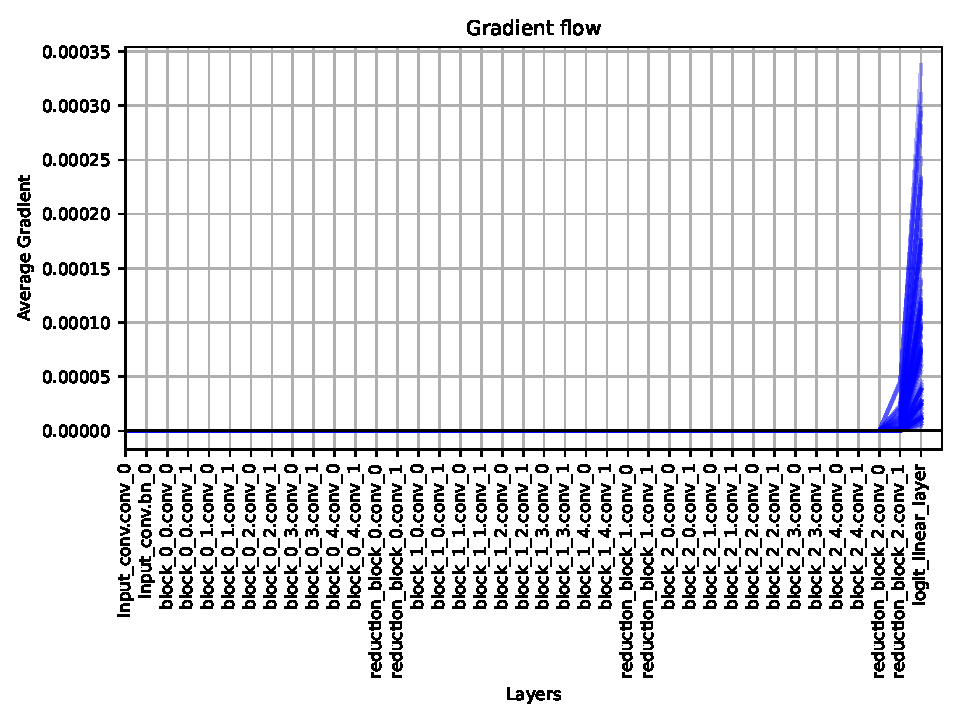
\includegraphics[width=\linewidth]{figures/vgg38_experiment_grad_flow.pdf}
    \caption{Gradient Flow on VGG38}
    \label{fig:grad_flow_38}
\end{figure}
}
}

%% Question Figure 4:
\newcommand{\questionFigureFour} {
\youranswer{Question Figure 4 - Replace this image with a figure depicting the training curves for the model with the best performance \textit{across experiments you have available (you don't need to run the experiments for the models we already give you results for)}. Edit the caption so that it clearly identifies the model and what is depicted.
%
\begin{figure}[t]
    \centering
    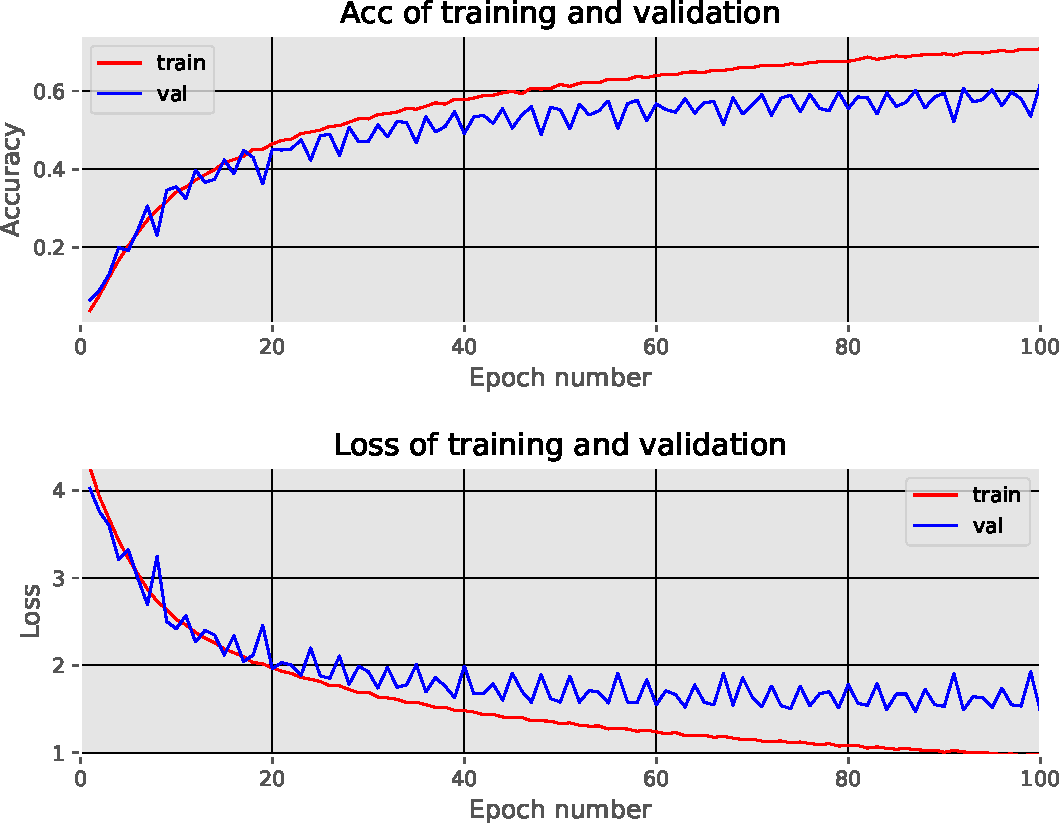
\includegraphics[width=\linewidth]{figures/BN+RC_training_curve.pdf}
    \caption{Training curves for BN+RC network with 1e-2 learning rate}
    \label{fig:grad_flow_bestModel}
\end{figure}
}
}

%% Question Figure 5:
\newcommand{\questionFigureFive} {
\youranswer{Question Figure 5 - Replace this image with a figure depicting the average gradient across layers, for the model with the best performance \textit{across experiments you have available (you don't need to run the experiments for the models we already give you results for)}. Edit the caption so that it clearly identifies the model and what is depicted.
%
\begin{figure}[t]
    \centering
    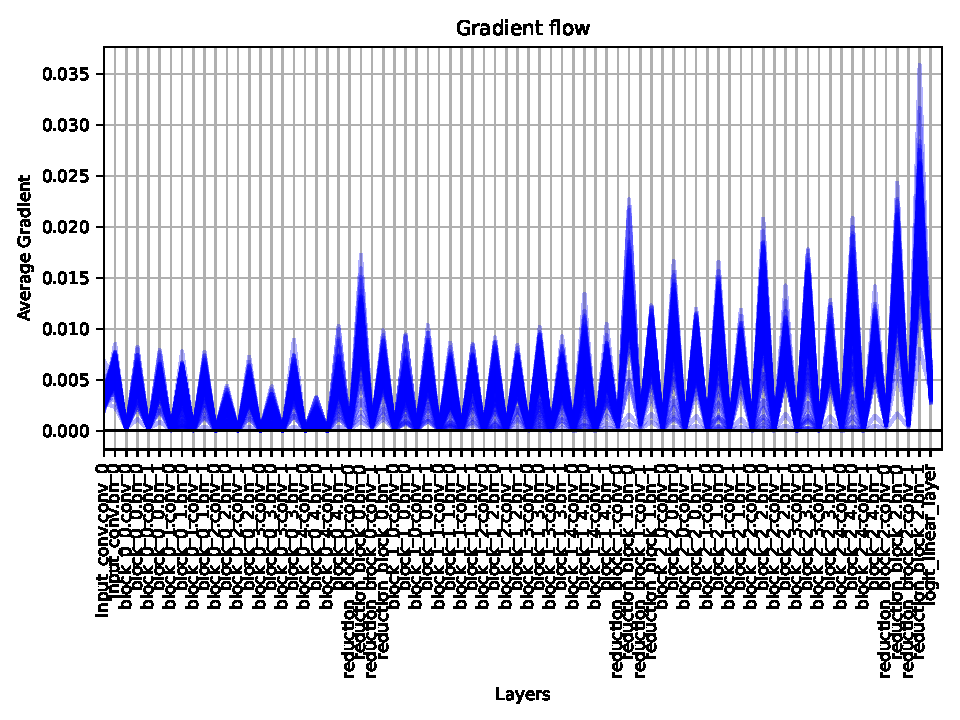
\includegraphics[width=\linewidth]{figures/BN+RC_1e-2.pdf}
    \caption{Gradient Flow on BN+RC network with 1e-2 learning rate}
    \label{fig:grad_flow_bestModel}
\end{figure}
}
}

%% - - - - - - - - - - - - TABLES - - - - - - - - - - - - 

%% Question Table 1:
\newcommand{\questionTableOne} {
\youranswer{
Question Table 1 - Fill in Table 1 with the results from your experiments on 
\begin{enumerate}
    \item \textit{VGG38 BN (LR 1e-3)}, and 
    \item \textit{VGG38 BN + RC (LR 1e-2)}.
\end{enumerate}
%
\begin{table*}[t]
    \centering
    \begin{tabular}{lr|ccccc}
    \toprule
        Model                   & LR   & \# Params & Train loss & Train acc & Val loss & Val acc \\
    \midrule
        VGG08                   & 1e-3 & 60 K      &  1.74      & 51.59     & 1.95     & 46.84 \\
        VGG38                   & 1e-3 & 336 K     &  4.61      & 00.01     & 4.61     & 00.01 \\
        VGG38 BN                & 1e-3 & 339 K     &  1.67      & 52.61     & 1.94     & 47.28 \\
        VGG38 RC                & 1e-3 & 336 K     &  1.33      & 61.52     & 1.84     & 52.32 \\
        VGG38 BN + RC           & 1e-3 & 339 K     &  1.26      & 62.99     & 1.73     & 53.76 \\
        VGG38 BN                & 1e-2 & 339 K     &  1.70      & 52.28     & 1.99     & 46.72 \\
        VGG38 BN + RC           & 1e-2 & 339 K     &  \textbf{0.97}      & \textbf{70.80}     & \textbf{1.48}     & \textbf{61.72} \\
    \bottomrule
    \end{tabular}
    \caption{Experiment results (number of model parameters, Training and Validation loss and accuracy) for different combinations of VGG08, VGG38, Batch Normalisation (BN), and Residual Connections (RC), LR is learning rate.}
    \label{tab:CIFAR_results}
\end{table*} 
}
}

%% END of YOUR ANSWERS
%% END of YOUR ANSWERS



%% Do not change anything in this file. Add your answers to mlp-cw1-questions.tex



\begin{document} 

\twocolumn[
\mlptitle{MLP Coursework 2}
\centerline{\studentNumber}
\vskip 7mm
]

\begin{abstract} 
Deep neural networks have become the state-of-the-art 
in many standard computer vision problems thanks to their powerful
representations and availability of large labeled datasets.
While very deep networks allow for learning more levels of abstractions in their layers from the data,
training these models successfully is a challenging task
due to problematic gradient flow through the layers, 
known as vanishing/exploding gradient problem.
In this report, we first analyze this problem in VGG models
with 8 and 38 hidden layers on the CIFAR100 image dataset, 
by monitoring the gradient flow during training. 
We explore known solutions to this problem including batch
normalization or residual connections, and explain their theory
and implementation details. 
Our experiments show that batch normalization and residual connections effectively
address the aforementioned problem and hence enable a deeper model to outperform
shallower ones in the same experimental setup.
\end{abstract} 

\section{Introduction}
\label{sec:intro}
Despite the remarkable progress of deep neural networks in image classification problems~\cite{simonyan2014very, he2016deep}, training very deep networks is a challenging procedure.
One of the major problems is the Vanishing Gradient Problem (VGP), a phenomenon where the gradients of the error function with respect to network weights shrink to zero, as they backpropagate to earlier layers, hence preventing effective weight updates. 
This phenomenon is prevalent and has been extensively studied in various deep neural networks including feedforward  networks~\cite{glorot2010understanding},  RNNs~\cite{bengio1993problem}, and CNNs~\cite{he2016deep}. 
Multiple solutions have been proposed to mitigate this problem by using weight initialization strategies~\cite{glorot2010understanding},
activation functions~\cite{glorot2010understanding}, input normalization~\cite{bishop1995neural},
batch normalization~\cite{ioffe2015batch}, and shortcut connections \cite{he2016deep, huang2017densely}.

This report focuses on diagnosing the VGP occurring in the VGG38 model and addressing it by implementing two standard solutions.
In particular, we first study a ``broken'' network in terms of its gradient flow, norm of gradients with respect to
its weights for each layer and contrast it to ones in the healthy VGG08 to pinpoint the problem.
Next, we review two standard solutions for this problem,  batch normalization (BN)~\cite{ioffe2015batch} and residual connections (RC)~\cite{he2016deep} in detail and discuss how they can address the gradient problem.
We first incorporate batch normalization (denoted as VGG38+BN), residual connections (denoted as VGG38+RC),  and their combination (denoted as VGG38+BN+RC) to the given VGG38 architecture.
We train the resulting three configurations, and VGG08 and VGG38 models on CIFAR-100 dataset and present the results.
The results show that though separate use of BN and RC does mitigate the vanishing/exploding gradient problem, therefore enabling effective training of the VGG38 model, the best results are obtained by combining both BN and RC.

%


\section{Identifying training problems of a deep CNN}
\label{sec:task1}

\begin{figure}[t]
    \begin{subfigure}{\linewidth}
        \centering
        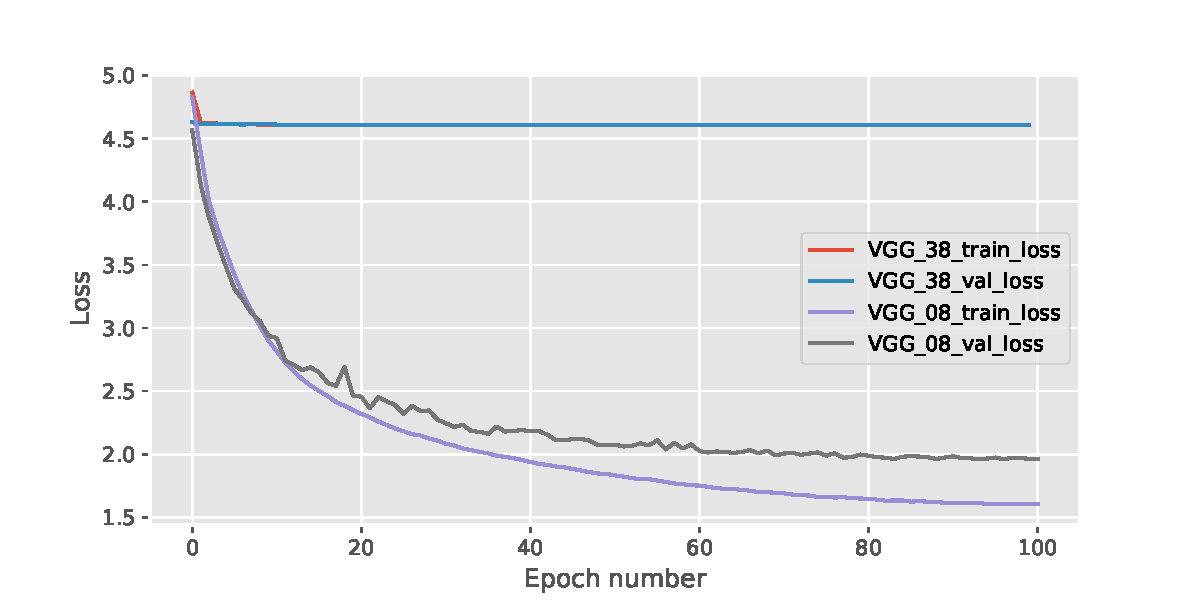
\includegraphics[width=\linewidth]{figures/loss_plot.pdf}
        \caption{Loss per epoch}
        \label{fig:loss_curves}
    \end{subfigure}

    \begin{subfigure}{\linewidth}
        \centering
        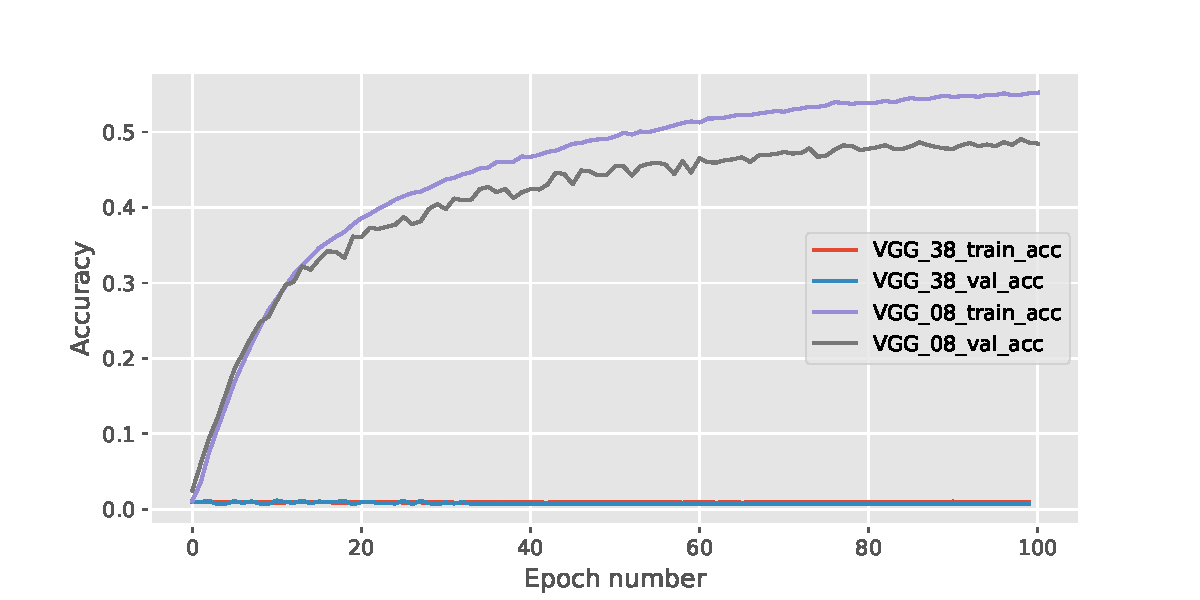
\includegraphics[width=\linewidth]{figures/accuracy_plot.pdf}
        \caption{Accuracy per epoch}
        \label{fig:acc_curves}
    \end{subfigure}
    \caption{Training curves for VGG08 and VGG38}
    \label{fig:curves}
\end{figure}

\begin{figure}[t]
    \centering
    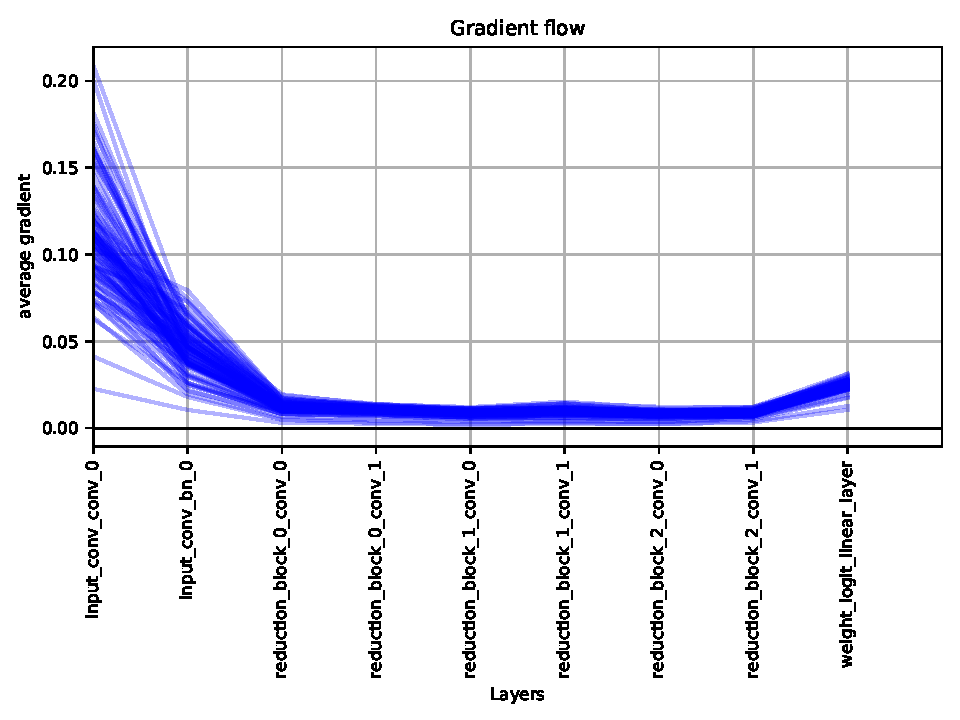
\includegraphics[width=\linewidth]{figures/grad_flow_vgg08.pdf}
    \caption{Gradient flow on VGG08}
    \label{fig:grad_flow_08}
\end{figure}

\questionFigureThree

Concretely, training deep neural networks typically involves three steps: forward
pass, backward pass (or backpropagation algorithm~\cite{rumelhart1986learning}) and weight update.
The first step involves passing the input $\bx^0$ to the network and producing 
the network prediction and also the error value.
In detail, each layer takes in the output of the previous layer and applies
a non-linear transformation:
\begin{equation}
\label{eq.fprop}
\bx^{(l)} = f^{(l)}(\bx^{(l-1)}; W^{(l)})    
\end{equation} 
where $(l)$ denotes the $l$-th layer in $L$ layer deep network,
$f^{(l)}(\cdot,W^{(l)})$ is a non-linear transformation for layer $l$, and $W^{(l)}$ are the weights of layer $l$.
For instance, $f^{(l)}$ is typically a convolution operation followed by an activation function in convolutional neural networks.
The second step involves the backpropagation algorithm, where we calculate the gradient of an error function $E$ (e.g. cross-entropy) for each layer's weight as follows:

\begin{equation}
    \label{eq.bprop}
\frac{\partial E}{\partial W^{(l)}} = \frac{\partial E}{\partial \bx^{(L)}} \frac{\partial \bx^{(L)}}{\partial \bx^{(L-1)}} \dots \frac{\partial \bx^{(l+1)}}{\partial \bx^{(l)}}\frac{\partial \bx^{(l)}}{\partial W^{(l)}}.
\end{equation}

This step includes consecutive tensor multiplications between multiple
partial derivative terms.
The final step involves updating model weights by using the computed 
$\frac{\partial E}{\partial W^{(l)}}$ with an update rule.
The exact update rule depends on the optimizer.

A notorious problem for training deep neural networks is the vanishing/exploding gradient
problem~\cite{bengio1993problem} that typically occurs in the backpropagation step when some of partial gradient terms in Eq.~\ref{eq.bprop} includes values larger or smaller than 1.
In this case, due to the multiple consecutive multiplications, the gradients w.r.t. weights
can get exponentially very small (close to 0) or very large (close to infinity) and
prevent effective learning of network weights.


%


Figures~\ref{fig:grad_flow_08} and \ref{fig:grad_flow_38} depict the gradient flows through
VGG architectures \cite{simonyan2014very} with 8 and 38 layers respectively,
trained and evaluated for a total of 100 epochs on the 
CIFAR100 dataset. \questionOne.


\section{Background Literature}
\label{sec:lit_rev}
In this section we will highlight some of the most influential
papers that have been central to overcoming the VGP in
deep CNNs.

\paragraph{Batch Normalization}\cite{ioffe2015batch}
BN seeks to solve the  problem of 
internal covariate shift (ICS), when distribution of each layer’s 
inputs changes during training, as the parameters of the previous layers change. 
The authors
argue that without batch normalization, the distribution of
each layer’s inputs can vary significantly due to the 
stochastic nature of randomly sampling mini-batches from your
training set. Layers in the network hence must continuously
adapt to these high variance distributions which hinders the
rate of convergence gradient-based optimizers. This optimization
problem is exacerbated further with network depth due
to the updating of parameters at layer $l$ being dependent on
the previous $l-1$ layers.

It is hence beneficial to embed the normalization of
training data into the network architecture after work from
LeCun \emph{et al.} showed that training converges faster with
this addition \cite{lecun2012efficient}. Through standardizing
the inputs to each layer, we take a step towards achieving
the fixed distributions of inputs that remove the ill effects
of ICS. Ioffe and Szegedy demonstrate the effectiveness of
their technique through training an ensemble of BN
networks which achieve an accuracy on the ImageNet classification
task exceeding that of humans in 14 times fewer
training steps than the state-of-the-art of the time.
It should be noted, however, that the exact reason for
BN’s effectiveness is still not completely understood and it is 
an open research question~\cite{santurkar2018does}.



\paragraph{Residual networks (ResNet)}\cite{he2016deep} A well-known way of mitigating the VGP is proposed by He~\emph{et al.} in \cite{he2016deep}. In their paper, the authors depict the error curves of a 20 layer and a 56 layer network to motivate their method. Both training and testing error of the 56 layer network are significantly higher than of the shallower one.

\questionTwo.

Residual networks, colloquially
known as ResNets, aim to alleviate VGP through the
incorporation of skip connections that bypass the linear
transformations into the network architecture. 
The authors argue that this new mapping is significantly easier
to optimize since if an identity mapping were optimal, the
network could comfortably learn to push the residual to
zero rather than attempting to fit an identity mapping via
a stack of nonlinear layers. 
They bolster their argument
by successfully training ResNets with depths exceeding
1000 layers on the CIFAR10 dataset.
Prior to their work, training even a 100-layer was accepted
as a great challenge within the deep learning community.
The addition of skip connections solves the VGP through
enabling information to flow more freely throughout the
network architecture without the addition of neither extra
parameters, nor computational complexity.

\section{Solution overview}
\subsection{Batch normalization}

\questionThree.


\subsection{Residual connections}

Residual connections are another approach used in the state-of-the-art Residual Networks~\cite{he2016deep} to tackle the vanishing gradient problem.
Introduced by He et. al.~\cite{he2016deep}, a residual block consists of a
convolution (or group of convolutions) layer, ``short-circuited'' with an identity mapping.
More precisely, given a mapping $F^{(b)}$ that denotes the transformation of the block $b$ (multiple consecutive layers), $F^{(b)}$ is applied to its input
feature map $\bx^{(b-1)}$ as $\bx^{(b)} = \bx^{(b-1)} + {F}(\bx^{(b-1)})$.

Intuitively, stacking residual blocks creates an architecture where inputs of each blocks
are given two paths : passing through the convolution or skipping to the next layer. A 
residual network can therefore be seen as an ensemble model averaging every sub-network
created by choosing one of the two paths. The skip connections allow gradients to flow
easily into early layers, since 
\begin{equation}
    \frac{\partial \bx_{(b)}}{\partial \bx^{(b-1)}} = \mathbbm{1} + \frac{\partial{F}(\bx^{(b-1)})}{\partial \bx^{(b-1)}}
    \label{eq.grad_skip}
\end{equation} where $\bx^{(b-1)} \in \mathbb{R}^{H \times W \times C}$ and $\mathbbm{1}$ is a $\mathbb{R}^{H \times W \times C}$-dimensional tensor with entries 1. 
Importantly, $\mathbbm{1}$ prevents the zero gradient flow.


\section{Experiment Setup}

\questionFigureFour

\questionFigureFive

\questionTableOne

We conduct our experiment on the CIFAR-100 dataset \cite{krizhevsky2009learning},
which consists of 60,000 32x32 colour images from
100 different classes. The number of samples per class is balanced, and the
samples are split into training, validation, and test set while
maintaining balanced class proportions. In total, there are
47,500; 2,500; and 10,000 instances in the training, validation,
and test set, respectively. Moreover, we apply data
augmentation strategies (cropping, horizontal flipping) to
improve the generalization of the model.

With the goal of understanding whether BN or skip connections
help fighting vanishing gradients, we first test these
methods independently, before combining them in an attempt
to fully exploit the depth of the VGG38 model.

All experiments are conducted using the Adam optimizer with the default
learning rate (1e-3) -- unless otherwise specified, cosine annealing and a batch size of 100
for 100 epochs. 
Additionally, training images are augmented with random 
cropping and horizontal flipping.
Note that we do not use data augmentation at test time.
These hyperparameters along with the augmentation strategy are used
to produce the results shown in Figure~\ref{fig:curves}.

When used, BN is applied
after each convolutional layer, before the Leaky
ReLU non-linearity. 
Similarly, the skip connections are applied from 
before the convolution layer to before the final activation function
of the block as per Figure~2 of \cite{he2016deep}. 
Note that adding residual connections between the feature maps before and after downsampling requires special treatment, as there is a dimension mismatch between them. 
Therefore in the coursework, we do not use residual connections in the down-sampling blocks. However, please note that batch normalization should still be implemented for these blocks. 

\subsection{Residual Connections to Downsampling Layers}
\label{subsec:rescimp}

\questionFour.


\section{Results and Discussion}
\label{sec:disc}

\questionFive.

\section{Conclusion}
\label{sec:concl}
    
\questionSix.

\bibliography{refs}

\end{document} 





